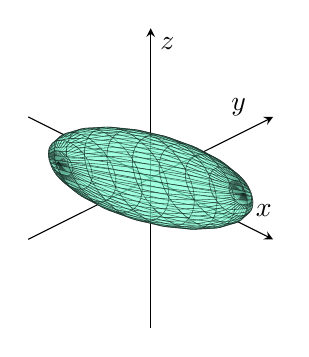
\begin{tikzpicture}
    \begin{axis}[%
        axis equal,
        width=8.5cm,
        colormap/blackwhite,
        height=8.5cm,
        axis lines = center,
        xlabel = {$x$},
        ylabel = {$y$},
        zlabel = {$z$},
        ticks=none,
        enlargelimits=0.3,
        view/h=45,
        scale uniformly strategy=units only,
        xmin=-3.5,
        xmax=3.5,
        ymin=-3.5,
        ymax=3.5,
        zmin=-3.5,
        zmax=3.5
    ]
    \addplot3[%
        opacity = 0.5,
        surf,
        line width=0.2pt,
        fill=Aquamarine,
        point meta=100,
        z buffer = sort,
        samples = 25,
        variable = \u,
        variable y = \v,
        domain = 0:180,
        y domain = 0:360,
    ]
    (
        {4/sqrt(2)*cos(u)*sin(v) + 0*sin(u)*sin(v) + 4/sqrt(2)*cos(v)}, 
        {-sqrt(2)*cos(u)*sin(v) - sqrt(2)*sin(u)*sin(v) + sqrt(2)*cos(v)}, 
        {0} 
    );
    \end{axis}
    \end{tikzpicture}